\documentclass{standalone}
\usepackage{tikz}
\usetikzlibrary{angles,quotes,math}

\begin{document}
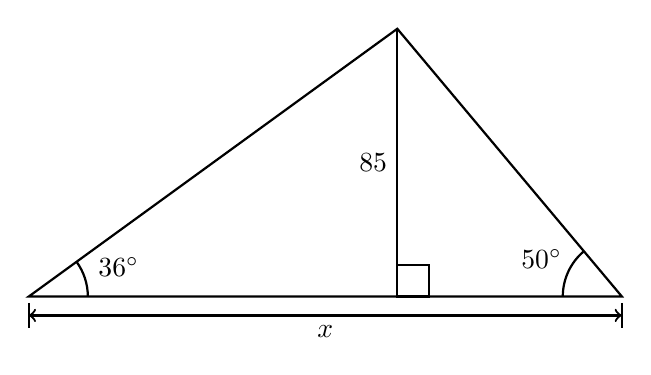
\begin{tikzpicture}[thick, scale=0.4]
  \coordinate (a) at (0,0);
  \coordinate (b) at (11.7,8.5);
  \coordinate (c) at (11.7,0);
  \coordinate (d) at ({11.7+7.13},0);
  \draw
  (a) pic["\(36^{\circ}\)", draw=black, -, angle eccentricity=1.6,
  angle radius=0.75cm] {angle=c--a--b} --
  (b) --
  (d) pic["\(50^{\circ}\)", draw=black, -, angle eccentricity=1.5,
  angle radius=0.75cm] {angle=b--d--a} -- cycle;
  \draw (c) -- node[left] {\(85\)} (b);
  % Right angle square
  \draw (c) rectangle ++(1,1);
  % x distance bars and arrows
  \draw (a)+(0,-0.2) -- ++(0,-1);
  \draw (d)+(0,-0.2) -- ++(0,-1);
  \draw[<->] (a)+(0,-0.6) -- node[midway,below] {\(x\)} ++({11.7+7.13},-0.6);
\end{tikzpicture}
\end{document}
